\section{引言}\label{sec:intro}


基础模型近期的进展极大地重塑了自然语言处理（NLP）和计算机视觉（CV）的研究与应用。相比之下，对于图结构数据开发类似成熟的自适应范式仍然相对有限 \cite{
devlin2019bert,
brown2020language, liu2023pretrain,
% radford2021learning,
% li2022blip,
% zhu2023minigpt4,
wang2023chatvideo,
zhang2023videollama}。这一差距至关重要，因为图是关系数据和结构数据的一种自然抽象，它们在分子发现、药物设计、推荐系统和科学建模等应用中扮演着核心角色 \cite{liu2023graph, zhang2023large, yang2023datacentric, rong2020selfsupervised, qian2023can, wang2023scientific}。因此，人们对通用图学习系统的兴趣日益增长，这类系统能够更好地在任务、领域和模态之间进行迁移。




\begin{figure}[!t]
    \centering
    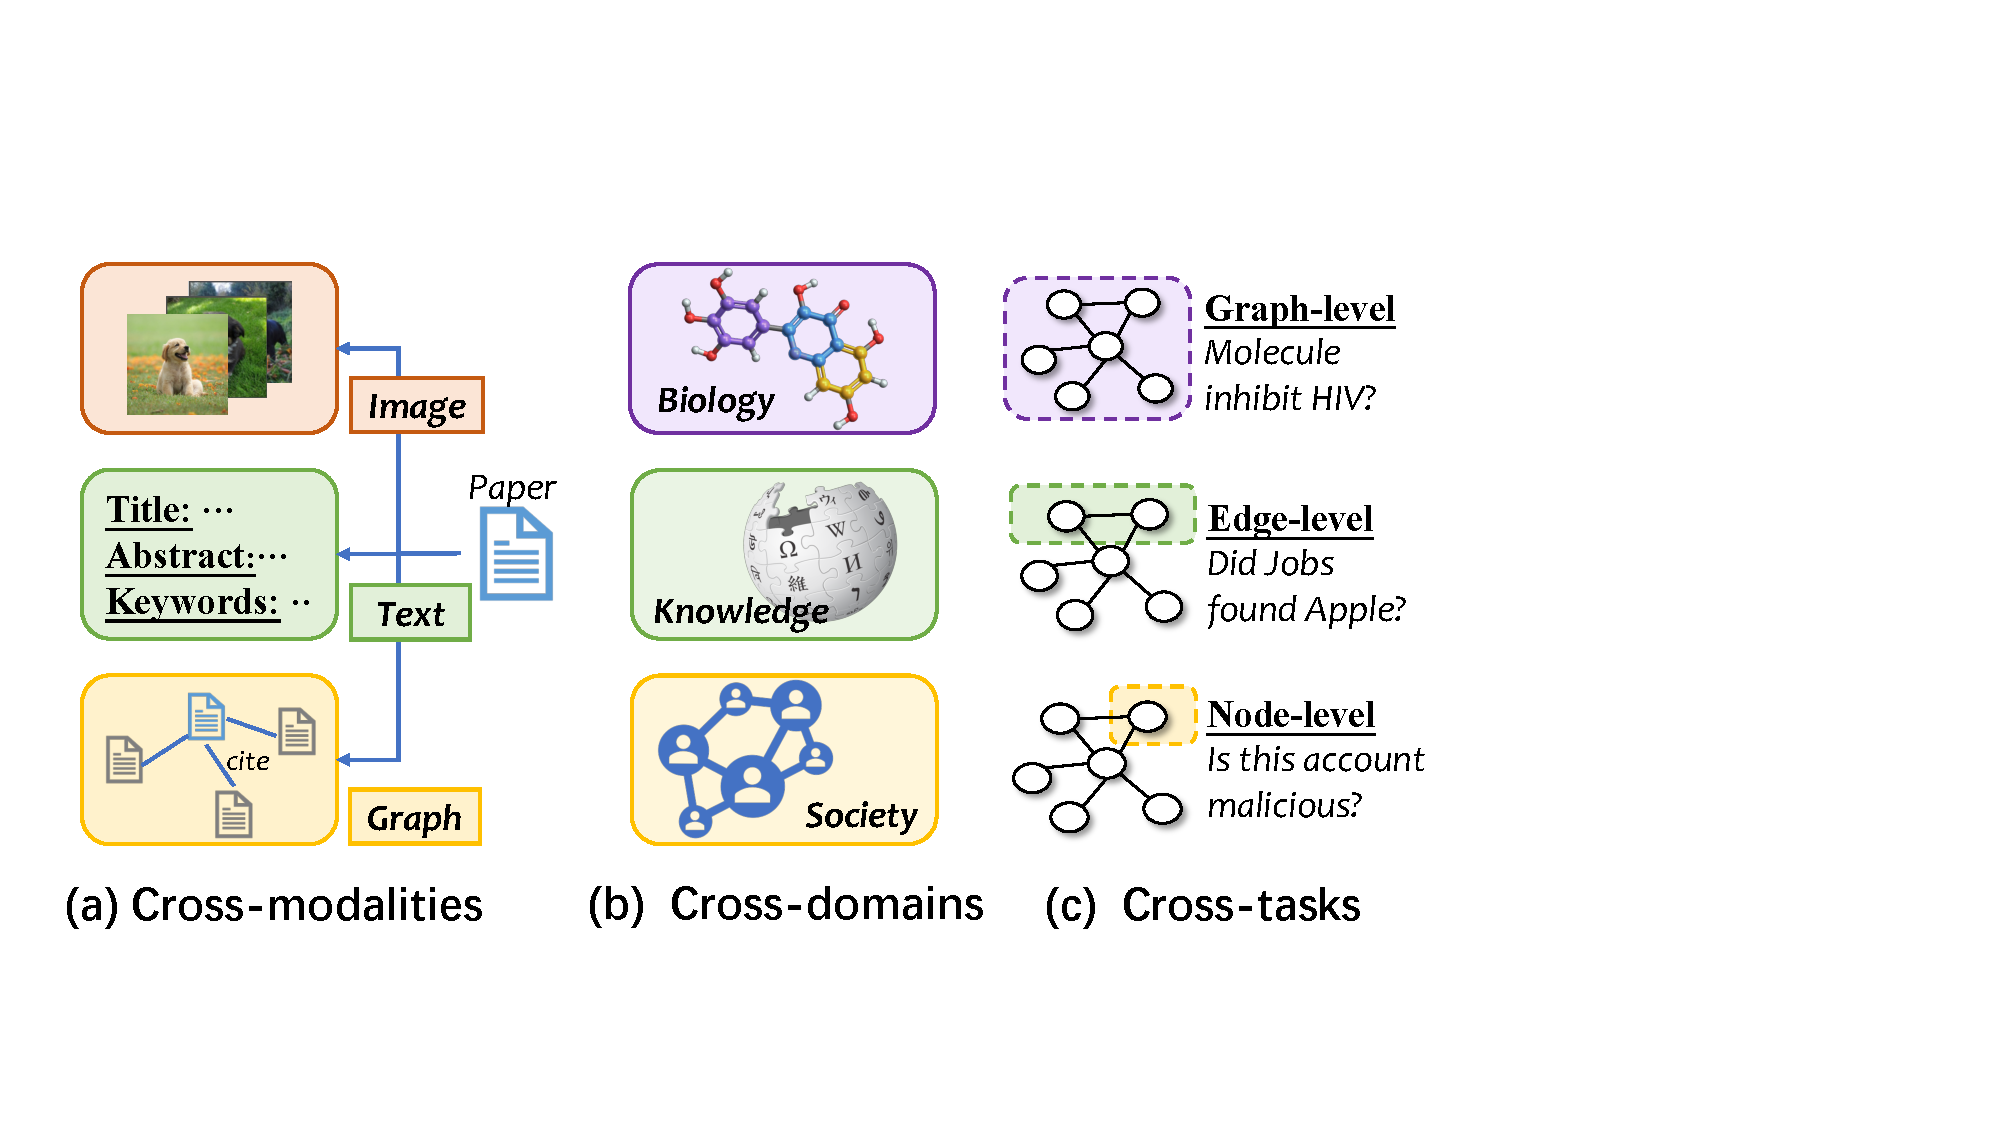
\includegraphics[width=0.45\textwidth]{pic/ThreeChallenges}
    \caption{迈向更通用图学习系统的三个反复出现的挑战：(a) 跨模态迁移，(b) 跨域迁移，和 (c) 跨任务迁移。}
    \label{fig:AGIProblems}
\end{figure}



然而，实现这一目标仍然困难重重。图 \ref{fig:AGIProblems} 突出显示了图学习研究中的三个反复出现的技术挑战。\textbf{\textit{(1) 模型如何跨模态泛化？}} 最近的多模态基础模型在文本和视觉输入的对齐和推理方面展现了强大的能力 \cite{
devlin2019bert,
% radford2021learning,
% li2022blip,
% zhu2023minigpt4,
zhang2023videollama,
brown2020language}。然而，在以图为中心的场景中，类似的进展仍然相当有限，特别是在图结构必须与文本、视觉或科学信号集成的情况下 \cite{li2023graphadapter}。
% he2023explanations,
% yoon2023multimodal,
% li2023graphadapter
% chen2023exploring
\textbf{\textit{(2) 模型如何跨域泛化？}} 迁移学习在许多机器学习设置中已经相当有效，但在图域之间迁移知识仍然具有挑战性，因为语义空间和结构模式都可能发生实质性变化 \cite{zhu2023graphcontrol, zhao2023graphglow}。这使得图域自适应成为一个困难且仍待解决的研穴问题。\textbf{\textit{(3) 模型如何跨任务泛化？}} 现有文献中的很大一部分集中在在同一图域内的不同任务之间迁移预训练的图知识，如节点分类、链路预测和图分类 \cite{sun2022gppt, liu2023graphprompt, sun2023all, fang2023universal, zhu2023sglpt, hu2020gptgnn, shirkavand2023deep, ge2023enhancing}。然而，与NLP和CV相比，面向标准化的实际评估和面向部署的图提示研究仍然相对有限。综合来看，这些观察表明，图提示不仅应被视为一种任务自适应技巧，更应被视为迈向更通用和可复用图学习系统的更广泛努力的一部分。
% Besides the above three foundation problems, Artificial General Intelligence has also encountered many social disputes. For example, training large foundation models consumes exorbitant amounts of energy and may yield unintended counterfactual outcomes \cite{liu2022ptuning, schick2021it}.


这些挑战使得参数高效自适应策略越来越受到关注 \cite{gao2021making, lester2021power}。其中，提示学习已成为一种无需重复更新所有模型参数即可使预训练模型适应下游任务的实用机制 \cite{qin2021learning, tsimpoukelli2021multimodal, liu2023pretrain}。提示学习通过修改输入或任务描述，使得下游问题更好地与预训练期间诱导的行为相一致。在许多场景中，这使得从业者能够以比完全微调少得多的可训练参数复用预训练模型 \cite{brown2020language, jiang2020how, lester2021power, shin2020autoprompt}。对于图学习而言，这一特性使提示学习成为一种有前景（虽然并非普遍足够）的任务自适应、跨域迁移和多模态交互机制。




% \begin{figure}[!t]
%     \centering
%     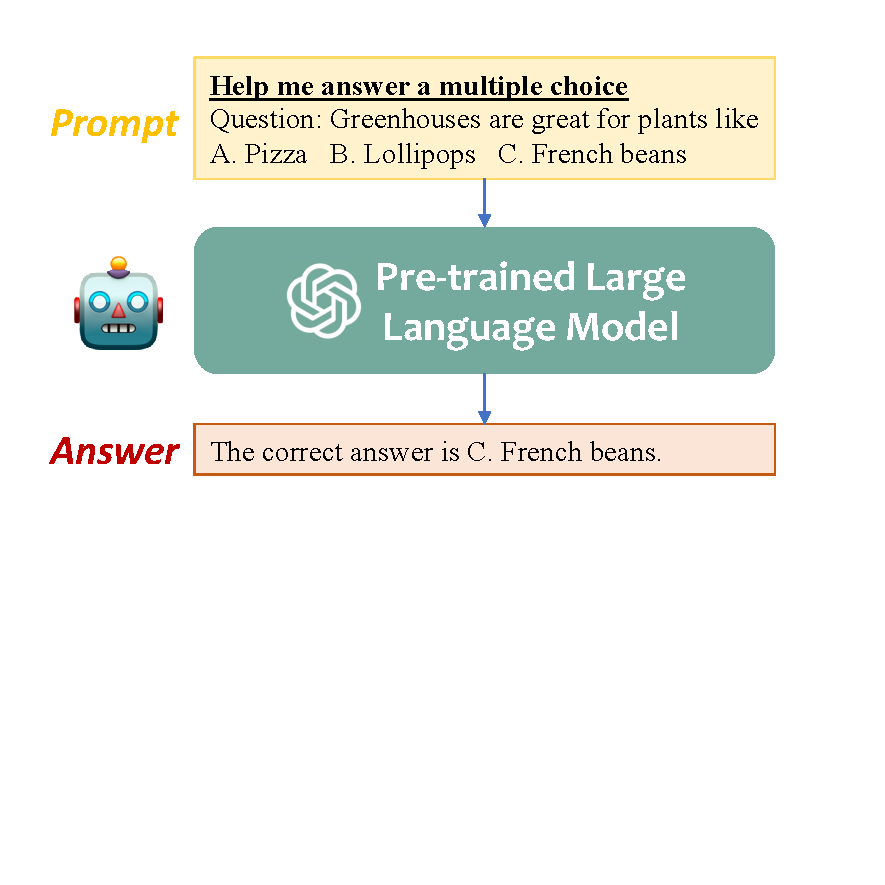
\includegraphics[width=0.45\textwidth]{pic/PromptExample.pdf}
%     \caption{An example of the language prompt. A textual prompt is designed to let the pre-trained large language model perform the multi-choice question-answering task.}
%     \label{fig:PromptExample}
% \end{figure}

\begin{figure}[!t]
\centering
\subfloat[语言提示]{
\label{fig:intro_lang_prompt}
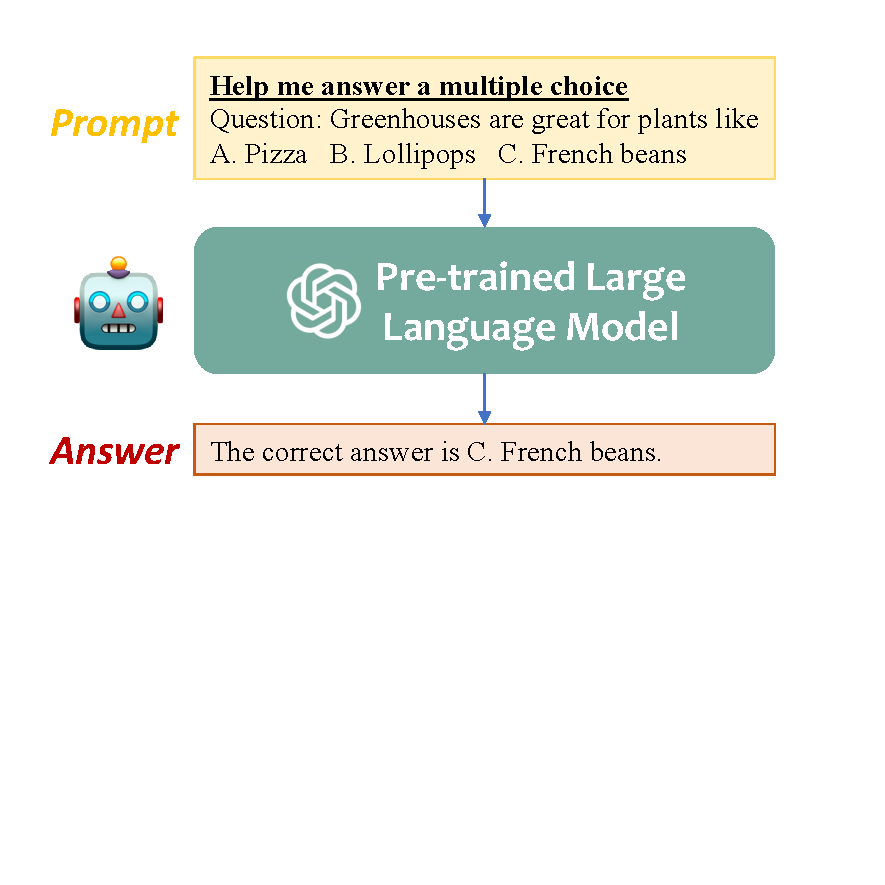
\includegraphics[width=0.36\textwidth]{pic/PromptExample.pdf}%
} \\
\subfloat[图提示 vs. 图微调]{
\label{fig:intro_graph_prompt}
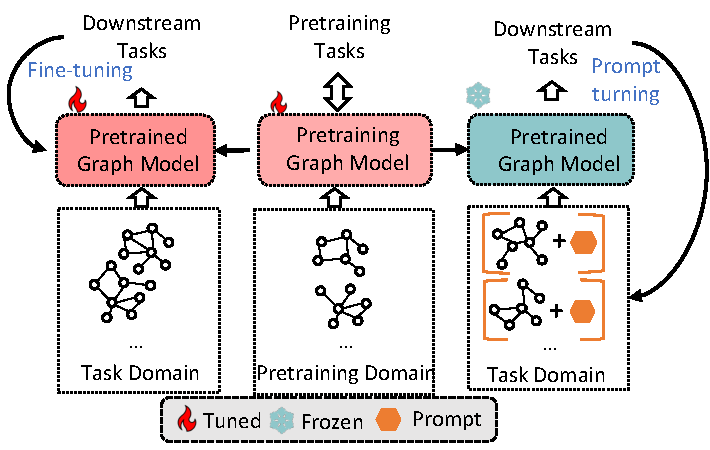
\includegraphics[width=0.44\textwidth]{pic/pt.pdf}%
}
\caption{语言提示与图提示的对比。一个文本提示被添加到原始输入中，以使预训练的大语言模型执行新任务（如选择题问答）。受语言提示的启发，图提示也可以用同样的方式与图结合使用。}\vspace{-3ex}
\label{fig:PromptExample}
\end{figure}


从表示的角度来看，几种数据模态可以通过图结构抽象重新解释。一个句子可以建模为依存图或标记交互图，一个图像可以表示为网格图或区域图。这种观点推动了成功的提示思想从语言和视觉领域向图学习的适配 \cite{sun2022gppt, liu2023graphprompt, sun2023all, fang2023universal, zhu2023sglpt, ma2023hetgpt, guo2023datacentric, chen2023ultradp, gong2023prompt}。


尽管图提示在一定程度上受NLP中提示技术的启发，但两者并不能直接类比 \cite{sun2023all}。\textbf{首先}，图提示的设计空间要丰富得多。在语言模型中，提示可能采取离散模板、软提示向量、前缀或指令式条件等形式 \cite{brown2020language, gao2021making}。然而，在图学习中，提示通常还涉及结构设计选择、插入机制和回答函数，而不仅仅是提示内容。\textbf{其次}，将下游图问题与预训练目标对齐通常比语言任务更困难 \cite{liu2023graphprompt, sun2023all}。一种典型的语言预训练任务如掩码词预测 \cite{devlin2019bert} 与许多下游任务共享一个相对直接的接口 \cite{liu2023pretrain}，而图任务涵盖节点级 \cite{grover2016node2vec}、边级 \cite{zhang2018link} 和图级目标 \cite{sun2020infograph, sun2021heterogeneous}，使得预训练的代理任务不那么直接可复用。\textbf{第三}，图提示通常比自然语言提示更难被非专业人员解释，因为它们的效果是通过图拓扑、特征变换和消息传递来调节的。这些差异使得图提示有必要按照其自身的术语来研究，而不是将其视为NLP提示的简单扩展。




图提示的文献近年来迅速扩展，但它仍然分散在不同的任务设置、图模态和自适应策略中。现有工作往往强调不同的观点，使得直接比较变得困难，并减缓了该领域知识系统化积累的进程。因此，本综述通过上述三个迁移挑战的视角，对图提示进行了结构化综述，同时也阐明了其与图预训练、图基础模型和多模态图学习的关系。为了组织这一领域，我们考虑以下研究问题（RQs）：

\begin{itemize}
    \item \textbf{RQ1：如何在一个统一的分析框架下组织现有的图提示方法？} 我们寻求一个通用词汇来比较在提示表示、插入机制和自适应目标方面存在差异的方法。
    \item  \textbf{RQ2：提示在图表示学习中扮演什么功能角色？} 我们研究图提示实际贡献了什么，它们如何与图学习器交互，以及为什么它们可能表现得与传统微调不同。


    \item  \textbf{RQ3：图提示和提示调优策略的主要设计维度是什么？} 我们探讨图提示是如何构建的，它们如何将下游任务与预训练目标对齐，以及它们在实践中如何优化。





    \item  \textbf{RQ4：如何在实际应用和软件生态系统中支持图提示？} 我们讨论了工具包（如ProG）、基准测试和可复用实现支持图提示的当前状态。

    \item  \textbf{RQ5：当前图提示研究存在哪些局限性，哪些未来方向最有前景？} 我们总结了开放挑战并概述了可能塑造该领域下一阶段发展的研究方向。


\end{itemize}




RQ1激发了用于分析图提示学习的统一框架。该框架将图提示分解为提示标记、标记结构和插入模式，从而为比较现有变体提供了一个稳定的视角。


RQ2关注通过灵活性和表达性的视角来理解提示与现有图模型的关系，从而更深入地理解图提示的作用。与许多NLP中的提示学习综述不同 \cite{liu2023pretrain}，这些综述主要将提示视为连接预训练和下游任务的机制，我们则将图提示讨论为与图学习器本身的建模能力交织在一起的机制。这一视角有助于阐明为什么提示在图领域是有前景的，以及它与传统微调方法的不同之处 \cite{hu2020strategies}。


RQ3激发了一种分类法，将代表性的图提示研究按照节点级、边级和图级设置进行组织，同时将它们与预训练目标的更广泛背景对齐。这种组织澄清了"预训练与提示"整体工作流程中的提示机制。

RQ4涉及图提示的支持生态系统。我们讨论了如ProG（提示图）\footnote{\url{https://github.com/sheldonresearch/ProG}}等工具包和精心策划的仓库 \footnote{\url{https://github.com/WxxShirley/Awesome-Graph-Prompt}}，这些提高了图提示研究者和实践者的可访问性、可复现性和可比性。

除这些问题外，本综述还进一步讨论了应用场景、当前挑战和未来研究方向，从而为图提示学习的发展描绘了更广泛的路线图（RQ5）。贡献总结如下：

\begin{itemize}
    \item \textbf{促进全面分析。} 我们开发了一个统一的框架来分析图提示学习，为提示标记、标记结构和插入模式提供了结构化的视图。
    \item \textbf{提示-模型视角。} 我们不仅将图提示视为任务适配器，还将其视为与图学习器的灵活性和表达性相互作用的机制。
    \item \textbf{图提示系统分类法。} 我们综合了代表性的图提示研究，并将其组织在"预训练与提示"的总体工作流程中。
    % \item \textbf{Quantitative and Qualitative Insights. } We conduct extensive experiments to evaluate different graph prompts and propose a new metric to evaluate how well a graph prompt reformulates graph data.
    \item \textbf{赋能图提示生态系统。} 我们总结了支持可复现图提示研究的工具包和社区资源。
    \item \textbf{描绘前进道路。} 我们对该领域的当前挑战和未来方向进行了详细讨论。
\end{itemize}


\textbf{路线图。} 本综述的其余部分组织如下：第 \ref{sec:method} 节介绍综述方法，第 \ref{sec:pre} 节介绍预备知识，第 \ref{sec:pretrain_method} 节介绍预训练方法，第 \ref{sec:ptask} 节介绍图模型提示方法。然后第 \ref{sec:pmodal} 节讨论多模态和多域设置中的图提示。第 \ref{sec:app} 节讨论图提示的潜在应用，第 \ref{sec:prog} 节介绍ProG。第 \ref{sec:dis} 节讨论当前挑战和未来方向。第 \ref{sec:con} 节总结综述并呈现作者贡献声明。
